\chapter{Design}
Our experiment with \texttt{malloc} and the experience we gained laid the foundation for the design of Explorant. Specifically, our experiment showed us the importance of building a temporal map that relates different segments of the codebase. When we were working with \texttt{malloc}, this map was created in our heads and on paper, however, Explorant was designed to help translate from important locations in the code to a readable state diagram of the program. To do this, we built a system that works on events organized inside modules.

\section{Events}
Explorant uses Events as a core building block. Events are similar to states in a FSM (Section \ref{sec:fsm}) however they are slightly more basic and less assuming. A real state in a FSM represents a unique global state of the program, though we do not have enough information to create such states without a much deeper understanding of the code. As such, we limit ourselves to discussing events. Each event can be effectively thought of as a breakpoint (though they are not implemented that way. See section \ref{sec:effaddrrec}). As the developer adds events on various lines throughout the program, we are able to create diagrams that relate these events and allow a developer to rapidly explore a trace in the form of a graph.

We envision that these events can serve as a form of accurate documentation that senior engineers can easily provide to junior engineers. We did this by allowing there to be two ways to define events: the first is through adding a source code annotation like: 
\begin{verbatim}
int main(){
    // [[{type:"event", name:"::entry"}]]
    printf("Hi!")
    return 0;
}
\end{verbatim}
The other option is to have the person who is exploring save all of their events to a JSON file which stays separate from the codebase but can easily be imported and exported from Explorant to allow for different profiles or investigation paths within the same codebase.


\section{Modules}
\label{sec:modules}
To achieve greater organization and categorization, we developed a module system. This system allows for the creation of namespaces, similar to popular programming languages. For example, instead of naming two ``entry'' points of functions as \texttt{func1\_entry} and \texttt{func2\_entry}, we can define a module with a unique name and a single parent, such as \texttt{add} being a child of \texttt{util}. In this case, the entry point of \texttt{add} can be specified as \texttt{add::entry} and the entry point of another function like \texttt{print} can be specified as \texttt{print::entry}. \\

\noindent This might look like the following in code:
\begin{verbatim}
#include <stdio.h>
// [[{type:"module", name:"util"}]]
// [[{type:"module", name:"print", parent_module:"util"}]]
// [[{type:"module", name:"add", parent_module:"util"}]]

int increment(int a){
    // Define a start event that gets expanded into ::util::add::entry
    // [[{type:"event", name:"add::entry"}]]
    a = a+1;
    return a;
}
void print_num(int a){
    // Define a start event that gets expanded into ::util::print::entry
    // [[{type:"event", name:"print::entry"}]]
    printf("val: %d\n", a);
}

int main(){
    // [[{type:"event", name:"::entry"}]]
    int a = increment(2);
    print_num(a);
    // [[{type:"event", name:"::exiting after printing the num"}]]
    return 0;
}
\end{verbatim}
\begin{figure}[!ht]
    \centering
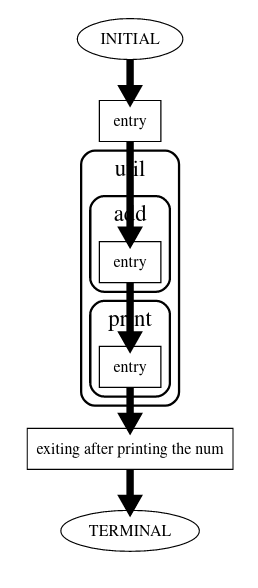
\includegraphics[scale=0.5]{modules}
    \caption{Graph of simple module system}
    \label{fig:modules}
\end{figure}

As you can see in figure \ref{fig:modules}, this sample code generated a simple graph containing multiple entry nodes all grouped into multiple different modules. This example is very contrived however it demonstrates multiple aspects of the module system. We can also see in figure \ref{fig:modules-collapsed} how these modules can be collapsed to simplify and hide complexity in the graph.


\begin{figure}[!ht]
\centering
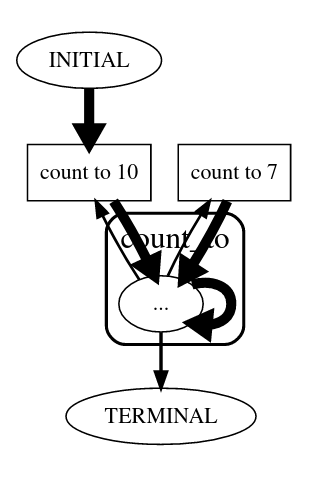
\includegraphics[scale=0.5]{modules-collapsed}
\caption{A collapsed module for a different program}
    \label{fig:modules-collapsed}
\end{figure}
We recommend keeping the number of modules to a minimum to prevent complicated and difficult-to-understand graphs. With many modules, our layout engine (Graphviz \cite{graphviz}) is more constrained during graph layout and this can cause the creation of many extra extremely long edges. However, careful placement of a few modules can make the graph much more legible and easily navigable. 

\section{Major components of the UX}
In this section, we will delve into the real implementation of major components of the software in order to provide concrete examples of how we solved many of the issues we encountered during our case study. Figure \ref{fig:graph-whole} shows the completed user interface that is actively examining a trace. In this figure, we can see that we have selected the \texttt{print} event and all of the components have been updated to highlight the event and show information about that event. 

\begin{figure}[!ht]
    \centering
    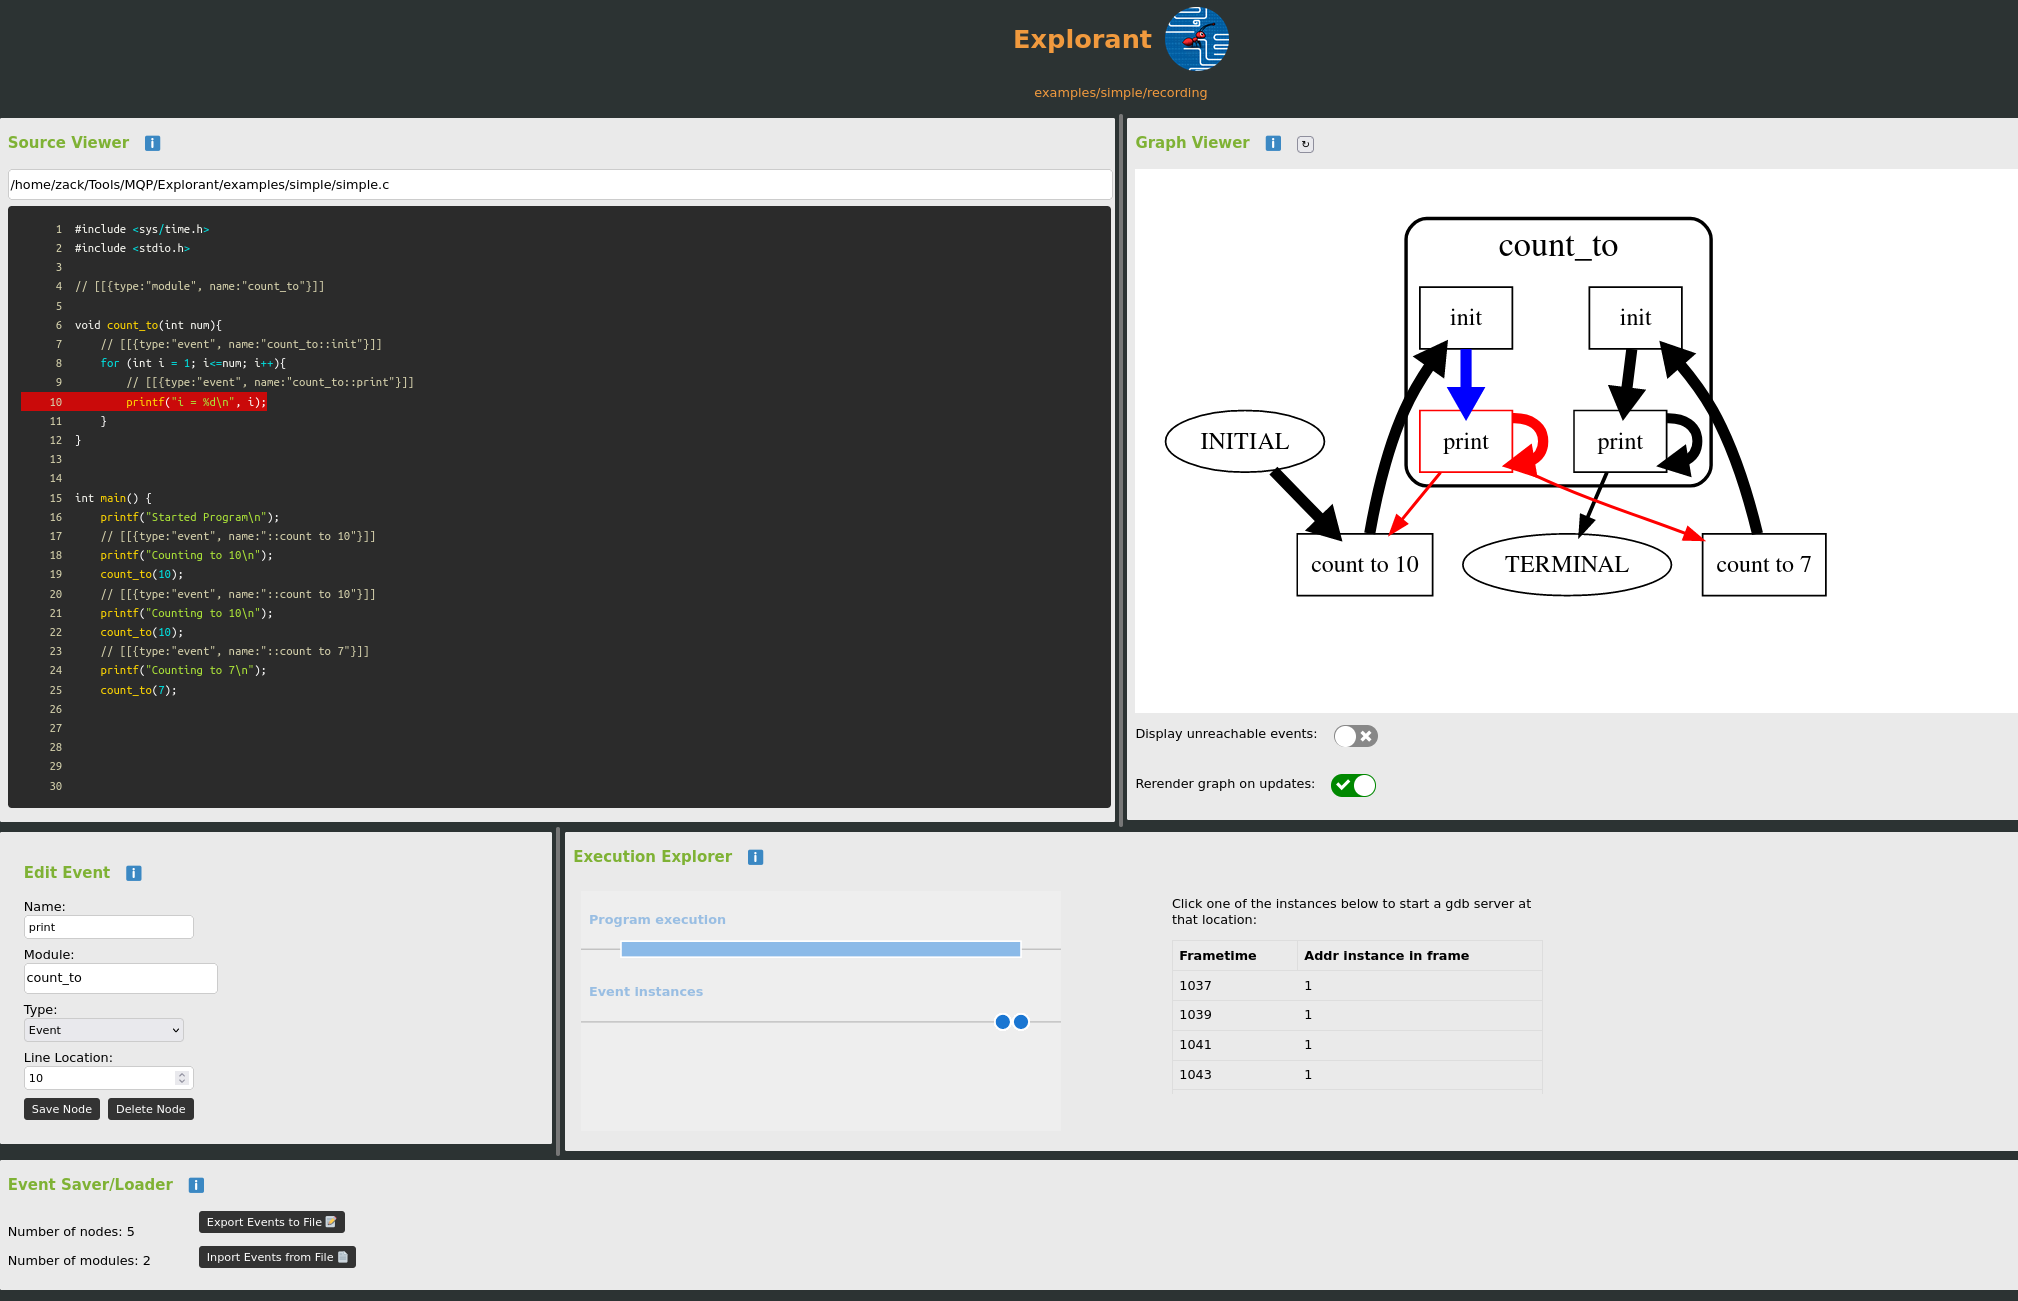
\includegraphics[scale=0.2]{design-whole}
    \caption{Image of the UI for Explorant}
    \label{fig:graph-whole}
\end{figure}

\subsection{Graph Viewer}
\begin{figure}[!ht]
    \centering
    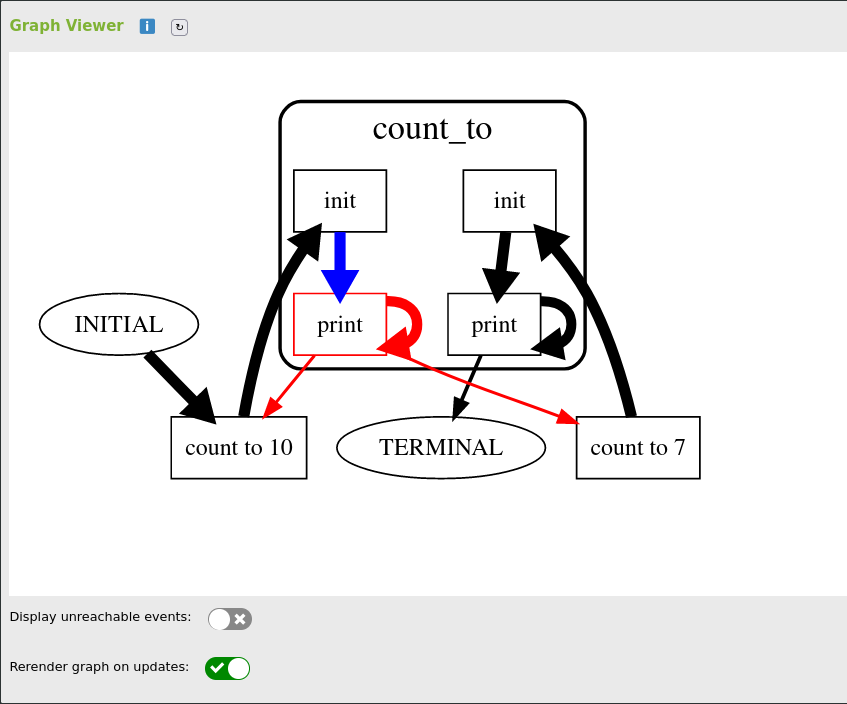
\includegraphics[scale=0.4]{design-graph}
    \caption{Image of the graph visualizer}
    \label{fig:graph}
\end{figure}
One of the most important components in Explorant is the graph viewer. The graph viewer describes the relationships between events across the entire execution of a trace. The graph viewer tries to convey as much information as possible. Some of the most important of these techniques are: 
\begin{itemize}
    \item The currently selected event is highlighted and all of its incoming and exiting nodes are colored. 
    \item The size of the edges are determined based on how probable that edge is to be traversed. 
    \item Events are grouped into modules (described in section \ref{sec:modules})
    \item Unreachable (Un-run) events can be toggled to only show the happy path that was actually executed during the trace.
    \item Hovering over an event shows what function it was defined in
\end{itemize}
You can see examples of these techniques in figure \ref{fig:graph} including the highlighted node \texttt{print}, the module \texttt{count\_to}, the varying sized edges, and program's entry and exit nodes, \texttt{INTIAL} and \texttt{TERMINAL}. 






\section{Source Viewer}
\begin{figure}[!ht]
    \centering
    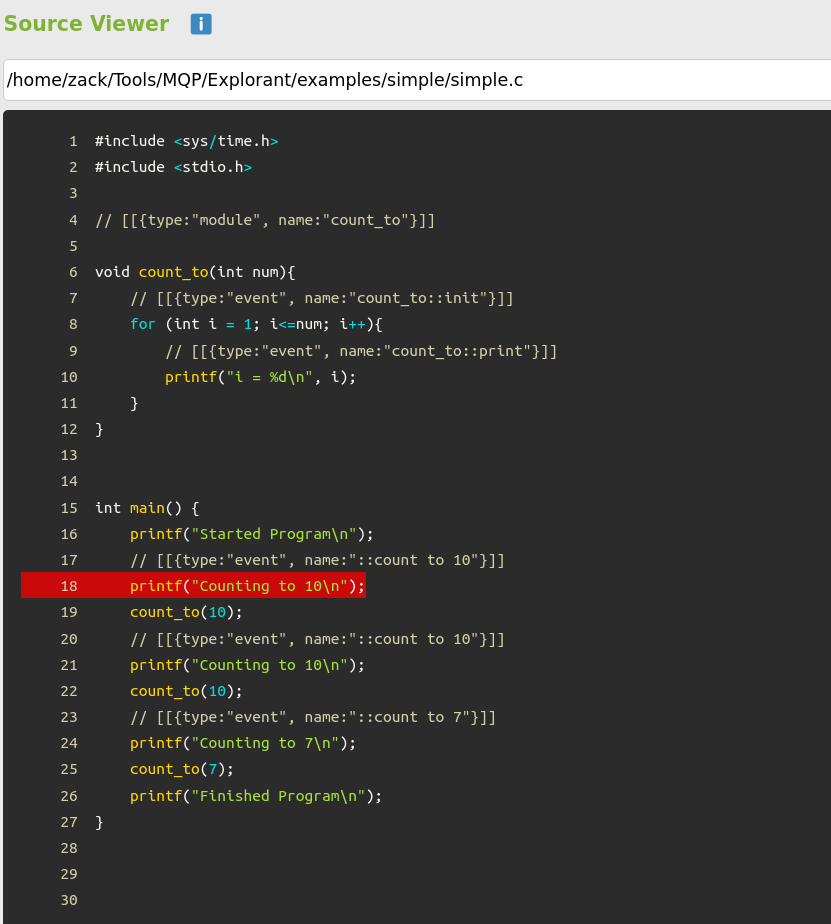
\includegraphics[scale=0.4]{design-source}
    \caption{Image of the source viewing component}
    \label{fig:graph-src}
\end{figure}
  Another critical design choice we made was to ensure that it is easy for the developer to relate the high-level state diagram to the source code easily. We addressed this by envisioning a simple source code viewer that contains features like syntax highlighting while also coloring the line with the currently selected event in red. This allows developers to easily move back and forth between the source code and the graph. The source viewer also can be right-clicked to allow the developer to add new events to the graph in real-time. You can see figure \ref{fig:graph-src} to see how this was implemented.

\section{Event Adding}
\begin{figure}[!ht]
    \centering
    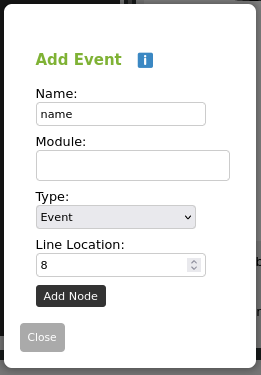
\includegraphics[scale=0.5]{design-adder}
    \caption{Image of the event adding component}
    \label{fig:graph-add}
\end{figure}
Our case study helped highlight how important real-time feedback and experimentation was to the onboarding experience. To ensure Explorant offered this kind of tight feedback loop, we allow the developer to add new events after a trace has already been recorded. We can leverage RR to replay the trace as if the new event had been there the whole time. This ensures that the developer has a tight feedback loop that does not entail recompiling and rerunning a program every time they want to experiment and add to the graph. Figure \ref{fig:graph-add} shows this component and how it allows the user to define events, determine what module they reside in, and what line they pertain to.  

\section{Execution Explorer}
\label{sec:exec-explorer}
\begin{figure}[!ht]
    \centering
    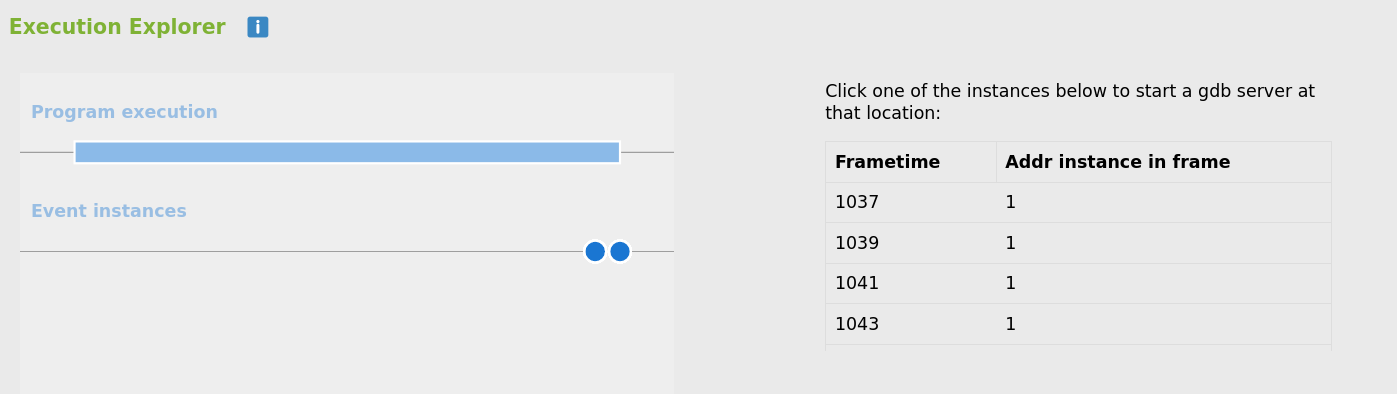
\includegraphics[scale=0.3]{design-explorer}
    \caption{Image of the execution explorer component}
    \label{fig:graph-exp}
\end{figure}
The last and perhaps most important constraint we considered when designing the UX of Explorant was the ability to dive deep when necessary. A debugger like GDB is capable of providing the developer with the means to get a very close look at a particular moment in time. As such, we allow the developer to see a list of every time an event was reached and when it occurred relative to the start of the program, and if they click on the particular instance of the event, it opens up gdb at that exact location. You can see figure \ref{fig:graph-exp} to see an image of how this was implemented. Note the timeline which shows all of the times the event was reached (with blue dots). The timeline also stacks some of these events because they occur so close together in time. 

\section{Graph Generation}
\label{sec:simplification}
Even with this GUI, A naive Explorant Event -> Graph Node mapping did not create understandable graphs. As such, we applied multiple filters to simplify the graphs for the developer. Without these filters, the graphs were rendered as giant nests of events, with each event having many edges in different parts of the codebase. The methods we employed were: a FSM miner (see section \ref{sec:fsm}), a module system (see section \ref{sec:modules}), and node-grouping techniques to simplify them.

\subsection{Synoptic}
\label{sec:synoptic}
The primary tool we leveraged to simplify the graph was Synoptic \cite{synoptic-site}, a finite state machine (FSM) miner. Developed by the University of Washington, Synoptic is described in their paper ``Leveraging Existing Instrumentation to Automatically Infer Invariant-Constrained Models'' \cite{synoptic}. Synoptic accepts a series of events that it uses to refine the graph. First, it creates a compact model where each node exists only once and is connected to all of the nodes that directly followed or preceded it. Then Synoptic mines invariants from the graph. In this context, an invariant is a statement such as ``x is always followed by y'', ``x always precedes y'', or ``x is never followed by y.''

By mining invariants, Synoptic is able to refine the graph and separate nodes that are used for multiple purposes (like \texttt{printf}) into multiple copies of the same node that represent different execution paths. This results in graphs with many more nodes but each node follows a clear and unique execution path. Consider the graph in figure \ref{fig:graph} where you can see how synoptic was able to break apart \texttt{print} and \texttt{init} in \texttt{count\_to} into two separate sets of nodes depending on whether or not they were called from \texttt{count to 10} or \texttt{count to 7}

\subsection{Grouping Strictly Sequential Nodes}
Grouping nodes that are strictly sequential also significantly simplified the graphs Explorant built. We define strictly sequential nodes A and B as having the only edge out of A directed to B and the only edge into B coming from A. Similarly, a set of nodes (A, B, C) is strictly sequential if A and B are strictly sequential and B and C are also strictly sequential. This technique is particularly useful for Synoptic graph simplification because Synoptic produces a large number of nodes and this helps to constrain and visually separate the graph. These groups are drawn with a dotted border. We created figure \ref{fig:seq-on-off} to show the effect of sequential grouping. These are two photos of the same graph, one with grouping enabled, and the other with it disabled. In this case, the grouping allows the user to quickly see the relationships between nodes that were otherwise hidden due to how they were displayed in the image on the left.

\begin{figure}[!ht]
\centering
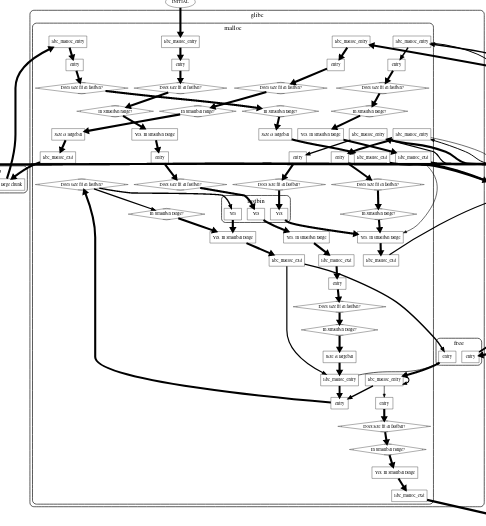
\includegraphics[scale=0.3]{simplification-sequential-off}
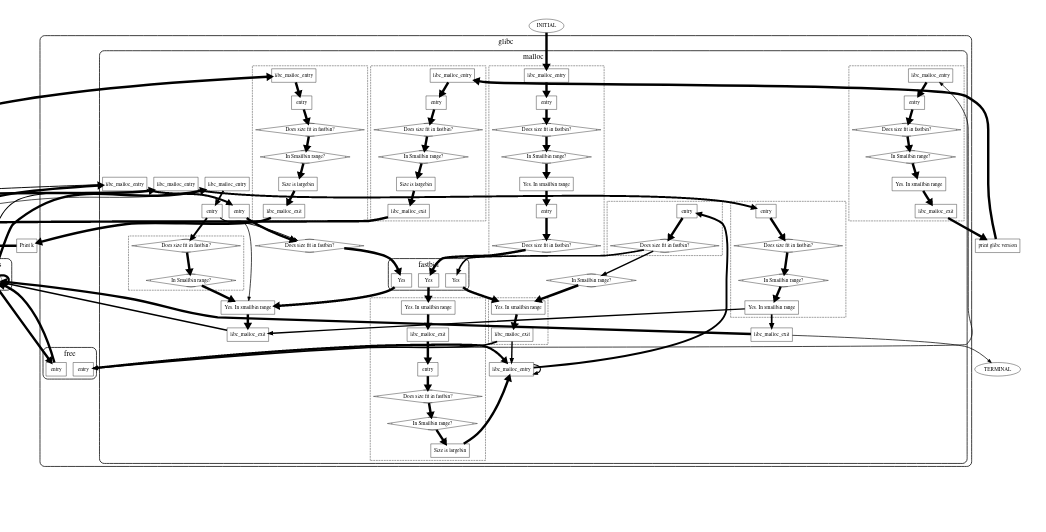
\includegraphics[scale=0.3]{simplification-sequential-on}
\caption{Off/On comparison showing strictly sequential grouping}
    \label{fig:seq-on-off}
\end{figure}


\section{Design Limitations}
\label{sec:design-limitations}

\noindent This design has a few major limitations that are worth examining:

\begin{description}
    \item[JIT compilation / self-modifying code] JITs \cite{jit} do not expose a standard method to access their location in the source code in the same way that static compilers provide DWARF data. This means that it is currently not feasible to instrument an arbitrary JIT compiler or code that it is running. Unfortunately, this means that many common languages like Java, Javascript, and Python will not work with Explorant.
\item[Macro heavy code] Macros hide a lot of information that DWARF data is unable to process as the macro is expanded in many locations and does not always translate to code very well. 
\item[Long-running programs] Because we must run the whole trace every time we rebuild the graph (in case an address was executed in a spot we didn't expect), working with long-running programs is difficult and painful. We could address this by either allowing the user to only analyze a certain time range within the trace or we could employ a much more advanced strategy where we instrument all function calls and then build heatmaps for where a new event could have been run and then only rerun those time segments. In either case, the current design does not allow for efficient manipulation of long-living programs. 
\item[Optimization levels] If a program is compiled with high optimization levels (like O3 in GCC \cite{gcc}) then functions can be inlined, loops can be unrolled, the DWARF data becomes harder to parse, and every line is no longer guaranteed to have assembly instructions associated with it. As such, this design means that the user must be sure to compile the program without optimization. This is particularly important because some programs like glibc cannot be compiled without optimization (glibc requires at least O2 \cite{glibco2}), meaning that sometimes annotations inside of \begin{tt}malloc\end{tt} do not behave as we expect them to. 
    \item[Browser dependent] The frontend is rendered in a browser (see section \ref{sec:frontend}). While this enables a fast development cycle, it also means that the final UI is much slower and heavier than a native app. 
\end{description}
